% ---------------------------------------------------------------------
% EG author guidelines plus sample file for EG publication using LaTeX2e input
% D.Fellner, v1.17, Sep 23, 2010


%\title[Automatic Proxy Geometry Generation]%
%      {Automatic Proxy Geometry Generation}

\title[Automatic Proxy Model Generation]%
      {Hybrid Client/Server Rendering with Automatic Proxy Model Generation}

% for anonymous conference submission please enter your SUBMISSION ID
% instead of the author's name (and leave the affiliation blank) !!
\author[short1043]{short1043}
%\author[J.\,O. Nygaard \& J. Mikkelsen]
%       {J.\,O. Nygaard$^{1}$
%        and J. Mikkelsen$^{1}$
%        \\
%         $^1$SINTEF ICT, Applied Mathematics, Norway
%       }

% ------------------------------------------------------------------------

% if the Editors-in-Chief have given you the data, you may uncomment
% the following five lines and insert it here
%
% \volume{27}   % the volume in which the issue will be published;
% \issue{1}     % the issue number of the publication
% \pStartPage{1}      % set starting page


%-------------------------------------------------------------------------
\begin{document}

\teaser{
  \centering
  \subfigure[Server-rendered (OpenGL)]{
    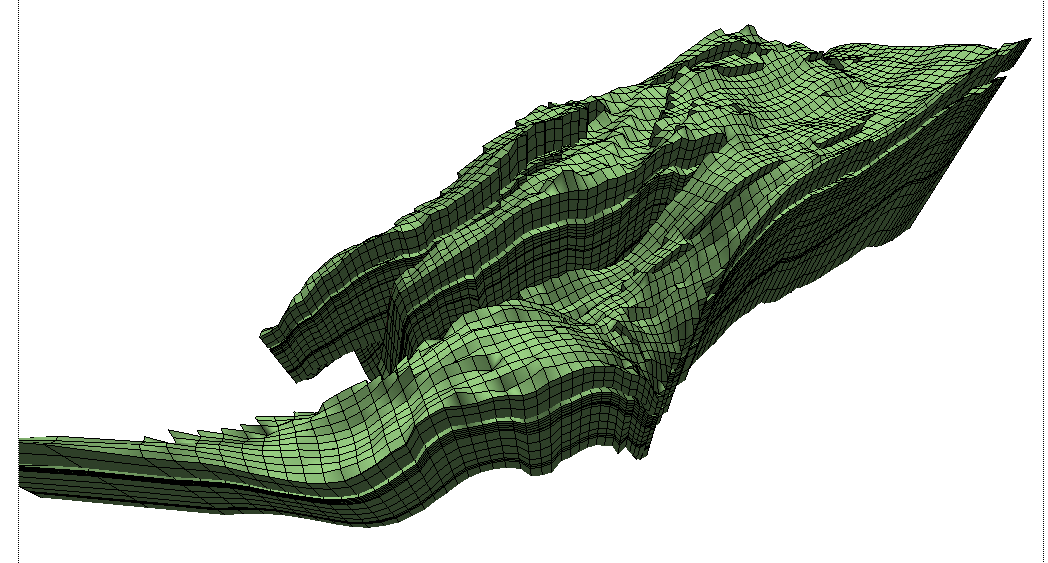
\includegraphics[width=0.32\linewidth, trim={1cm 1cm 1cm 1cm}, clip]{frviewb1.png}
  }
  \subfigure[Client-rendered (WebGL)]{
    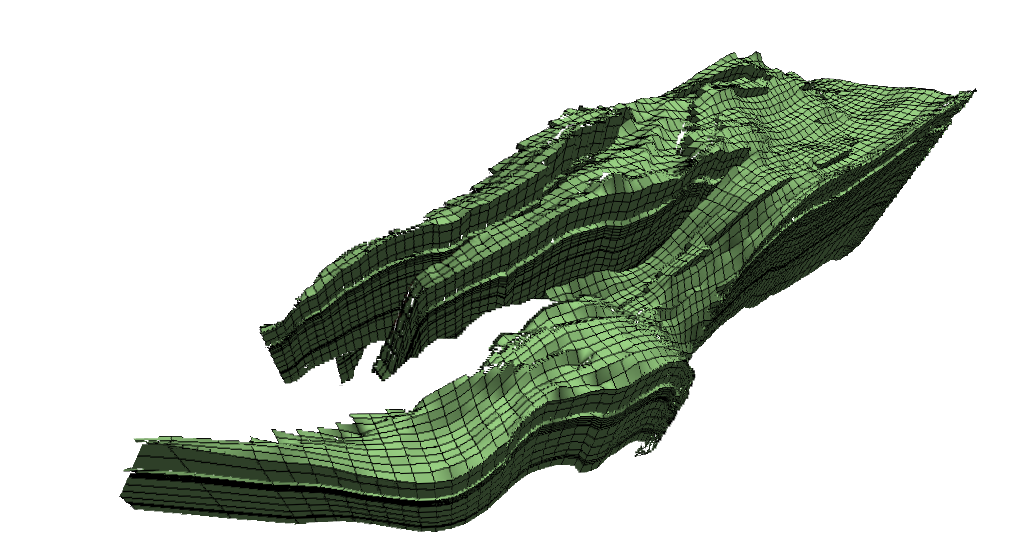
\includegraphics[width=0.32\linewidth, trim={0 1cm 0 1.5cm}, clip]{frviewb2.png}
  }
  \subfigure[Client-rendered (WebGL)]{
    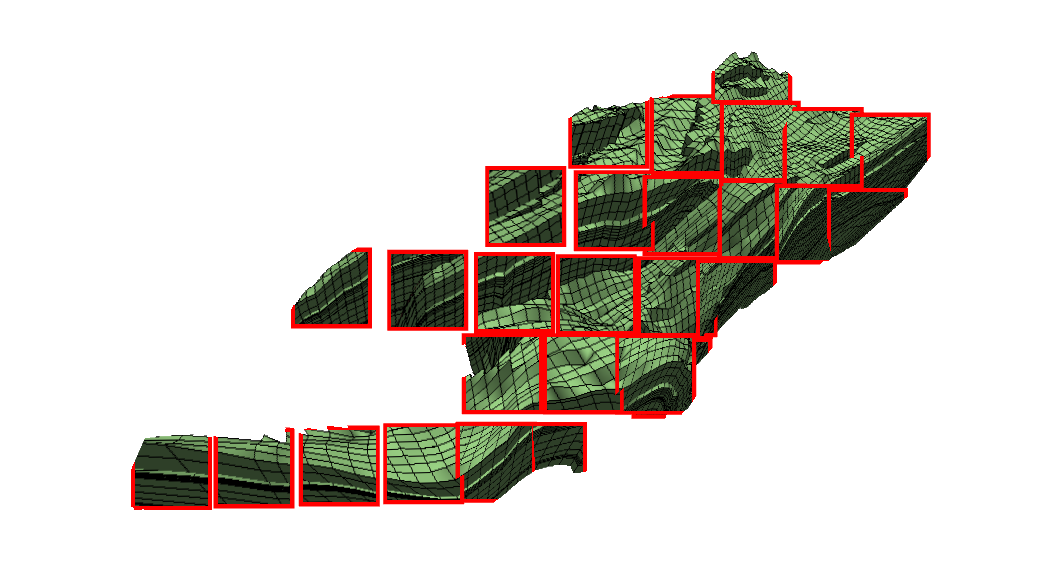
\includegraphics[width=0.32\linewidth, trim={0 1.5cm 0 2cm}, clip]{frviewb3.png}
    % The trim params: left lower right upper
  }
  \caption{\label{fig:FRView} The oil reservoir viewer YYYY~\cite{cloudviz},
  (name withheld for the double-blind review process) showing one
  server-rendered and two client-rendered images of automatically generated and
  slightly rotated proxy models.  For~(b), parameters are chosen to produce the
  best possible image, and in~(c) we want to highlight artifacts and
  implementational details. See the text for further discussion.}
}

\maketitle

\begin{abstract}
   We describe an algorithm and implementation of automatic proxy model
   generation for a client/server remote rendering setup. A {\em proxy model} is
   a light-weight version of a main 3D model that is cheaper to render and transfer. We
   automatically derive this from the main model. The client is typically a
   tablet, for which we only assume availability of WebGL and Javascript. The
   server makes use of OpenGL and a web server. When the rate of received
   server-rendered images deteriorate, the client renders the proxy model, which
   is computed from depth buffers bundled with rendered images from the
   server. This algorithm requires little modification of the application
   itself.
  % contribution sentence:
  %
  % The contribution of the work is the novel application of the depth buffer by-product of a rendering process to generate a simplified model of the rendered scene.
  % Husk: Skal vaere en blank linje nedenfor

\begin{classification} % according to http://www.acm.org/class/1998/
\CCScat{Computer Graphics}{I.3.5}{Computational Geometry and Object Modeling}{Geometric algorithms, languages, and systems}
% http://www.acm.org/about/class/ccs98-html
\end{classification}

\end{abstract}




%-------------------------------------------------------------------------
\section{Introduction}

Hand in hand with increasingly powerful rendering engines comes ever increasing
requirements on computational accuracy, power efficiency, data sizes, scaling
properties, etc. This is also reinforced by new cloud-based approaches and
wireless usage patterns. An effect of this is that interactivity still is a
difficult issue. We consider a client/server model for 3D rendering, addressing
latency, bandwidth and scaling problems in a novel way.

We introduce a {\em proxy model}, defined as a temporary model to be shown and
manipulated locally on a client while waiting for the appropriate image from a
connected server. Producing such proxy models can be difficult for many kinds of
3D data, like in our main case in which we have an oil reservoir viewer
(YYYY,~\cite{cloudviz}) that renders large {\em corner point grids}, together
with faults, oil wells, and more. See Figure~\ref{fig:FRView} above for an
example of both a full server-side rendering, and automatically generated proxy
models rendered in Google Chrome.
%
Our solution is to pass depth information from the server along with ordinary
rendered images. From this, a rudimentary 3D model is built, and with the RGB
image as a texture, this model can be manipulated and rendered on the client
while waiting for the next update from the server. If the client does not change
the position or orientation of the model too much, this proxy model rendering
integrates seamlessly with the slower stream of server-rendered frames.
%
Even if bandwidth and latency is not a problem, it may be desirable to let a
server of limited capacity serve many simultaneous users, hence limiting the
effective server time available for each one. Suitable scaling may still be
achieved using our solution. This is currently being commercialized in an
ongoing XXXX (name withheld for the double-blind review process) project.


%-------------------------------------------------------------------------
\subsection{Previous work}
\label{sec:prevWork}

Our approach has some similarities to {\em image based rendering} (IBR)
techniques, with the difference that an important IBR problem would be the
reconstruction of a depth map from images, while we have access to the full
depth map from a rendering pass.  Another way to use depth maps similar to what
we do, is for ``immersive streaming'', see \eg,~\cite{ibr}, where focus is on
depth map compression, an issue that we also consider. Another work
focused on similar streaming and geometry compression,
is~\cite{teler}. Also,~\cite{220764} contains some of the same ideas as our
work, with respect to image-based rendering acceleration.
%
Common to many IBR-algorithms is also that of stitching together 3D or 2.5D
point clouds. We could do this for our 2.5D maps fetched from the server, but it
is unclear if the benefit would outweigh the cost.
%
We are not aware of anybody else using depth maps exactly for our purpose, most
research seems to be focused on the retrieval of the depth map from images,
while we use an existing depth map to distill and render temporary geometry.
%
We observe that these 2.5D height maps are exactly what ``3D cameras''
(time-of-flight and other range image sensors) produce, but most authors
considering these are typically building more complex geometries before
visualization, see~\cite{IMM2009-05801}.


%-------------------------------------------------------------------------
\section{The auto proxy algorithm}

Since the depth buffer is a height map seen from the observer, it
does not contain information about occluded scene elements. Our approach assumes
that small transformations of this height map still will give good
approximations of the scene. In Figure~\ref{fig:2DheightmapRotated} below, a
sequence of three server-rendered images (thick lines) is shown, together with
intermediate client-rendered proxy models with different features that will be
discussed in Section~\ref{sec:client}.

\begin{figure}[htb]
  \centering
  \subfigure[Low frame rate]{
    %\begin{tikzpicture}[ scale=.25, show background rectangle]
\begin{tikzpicture}[scale=0.32, >=triangle 45, show background rectangle,
  declare function = {
    rotx(\x,\y,\th) = cos(\th)*\x - sin(\th)*\y; % NB! Cannot have space between parameters it seems!
    roty(\x,\y,\th) = sin(\th)*\x + cos(\th)*\y;
  }
  ]

  % View frustum
  \fill[fill=gray!20] (1, 0) -- (9, 0) -- (10, 5) -- (0, 5) -- cycle;
  % \clip (1, 0) -- (9, 0) -- (10, 5) -- (0, 5) -- cycle;
  % Clipping looks ok, but clipped content still expands bbox!! Solving this by reducing \pixels below from 13 to 11...


  % Defining some figure params

  \def \pixelwidth  {0.4}
  \def \pixelheight {0.3}
  \def \redstart    {2.2}
  \def \redpixels   {5}
  \def \pixels      {11}
  \def \linewidth   {1.25pt}
  \def \theta       {25}
  \def \cx          {5}
  \def \cy          {3}
  \def \rightcol    {red!100}
  \def \leftcolL    {blue!100}
  %\def \leftcolR    {red!100!blue!0} % Why doesn't this work?! (The color becomes white)
  \def \leftcolR    {red!100}


  % The scene, using same coordinate calculations as in the loop below

  \foreach \t in {0, ..., 4} {

    \pgfmathsetmacro\theta{25*\t}

    \ifthenelse{ \t = 0 \OR \t = 2 \OR \t = 4} {
      \def \rightcolToUse {\rightcol}
      \def \leftcolLToUse {\leftcolL}
      \def \leftcolRToUse {\leftcolR}
    }{
      \def \rightcolToUse {red!10}
      \def \leftcolLToUse {blue!10}
      \def \leftcolRToUse {red!10}
    }

    \pgfmathsetmacro\s{1}
    \pgfmathsetmacro\posx{0.5*(\s-1) + 2}
    \pgfmathsetmacro\posy{3.5 - 0.6*(\s-1)}
    \pgfmathsetmacro\posxRot{rotx(\posx-\cx, \posy-\cy, \theta)+\cx}
    \pgfmathsetmacro\posyRot{roty(\posx-\cx, \posy-\cy, \theta)+\cy}
    \coordinate (left) at ( \posxRot, \posyRot );
    
    \pgfmathsetmacro\s{\redpixels - 1}
    \pgfmathsetmacro\posx{0.5*(\s-1) + 2}
    \pgfmathsetmacro\posy{3.5 - 0.6*(\s-1)}
    \pgfmathsetmacro\posxRot{rotx(\posx-\cx, \posy-\cy, \theta)+\cx}
    \pgfmathsetmacro\posyRot{roty(\posx-\cx, \posy-\cy, \theta)+\cy}
    \coordinate (middle) at ( \posxRot, \posyRot );
    
    % The offset necessary for the red and green lines to meet properly
    \pgfmathsetmacro\redgreenintersection{3.5 -(0.6+0.2)*(\s-1)}
    
    \pgfmathsetmacro\s{\pixels}
    \pgfmathsetmacro\posx{0.5*(\s-1) + 2}
    \pgfmathsetmacro\posy{0.2*(\s-1) + \redgreenintersection}
    \pgfmathsetmacro\posxRot{rotx(\posx-\cx, \posy-\cy, \theta)+\cx}
    \pgfmathsetmacro\posyRot{roty(\posx-\cx, \posy-\cy, \theta)+\cy}
    \coordinate (right) at ( \posxRot, \posyRot );
    
    % The "server-rendered model"
    \fill[left color=\leftcolLToUse, right color=\leftcolRToUse, draw=none]
    (left) -- (middle) -- +(0, 3*\linewidth) -- ($ (left) + (0, 3*\linewidth) $) -- cycle;
    % Why is the factor 3 needed here?!?!
    % And why is there a (very thin) border?
    % And why is it not equally thick everywhere?

    \draw[\rightcolToUse, line width=\linewidth] (middle) -- (right);

  }


\end{tikzpicture}

  }
  \subfigure[Initial proxy model]{
    \begin{tikzpicture}[scale=0.32, >=triangle 45, show background rectangle,
  declare function = {
    rotx(\x,\y,\th) = cos(\th)*\x - sin(\th)*\y; % NB! Cannot have space between parameters it seems!
    roty(\x,\y,\th) = sin(\th)*\x + cos(\th)*\y;
  }
  ]

  % View frustum
  \fill[fill=gray!20] (1, 0) -- (9, 0) -- (10, 5) -- (0, 5) -- cycle;


  % Defining some figure params

  \def \pixelwidth  {0.4}
  \def \pixelheight {0.3}
  \def \redstart    {2.2}
  \def \redpixels   {5}
  \def \pixels      {11}
  \def \linewidth   {1.25pt}
  \def \cx          {5}
  \def \cy          {2.5}

  \pgfmathsetmacro\halfpixelwidth{0.5*\pixelwidth}


  \foreach \frame in {0} {  % , ..., 4} {
    \pgfmathsetmacro\theta{25*\frame}

    \ifthenelse{ \frame = 0 \OR \frame = 2 \OR \frame = 4} {
      \def \rightcolToUse {red!100}
      \def \leftcolLToUse {blue!100}
      \def \leftcolRToUse {red!100}
    }{
      \def \rightcolToUse {red!10}
      \def \leftcolLToUse {blue!10}
      \def \leftcolRToUse {red!10}
    }
    
    \def \withSplats {1}
    \def \withLargeSplats {0}
    \def \withConstantWidthSplats {1}
    \def \withFragDepth {0}

        \pgfmathsetmacro\s{1}
    \pgfmathsetmacro\posx{0.5*(\s-1) + 2}
    \pgfmathsetmacro\posy{3.5 - 0.6*(\s-1)}
    \pgfmathsetmacro\posxRot{rotx(\posx-\cx, \posy-\cy, 0)+\cx}
    \pgfmathsetmacro\posyRot{roty(\posx-\cx, \posy-\cy, 0)+\cy}
    \coordinate (left) at ( \posxRot, \posyRot );
    
    \pgfmathsetmacro\s{\redpixels - 1}
    \pgfmathsetmacro\posx{0.5*(\s-1) + 2}
    \pgfmathsetmacro\posy{3.5 - 0.6*(\s-1)}
    \pgfmathsetmacro\posxRot{rotx(\posx-\cx, \posy-\cy, 0)+\cx}
    \pgfmathsetmacro\posyRot{roty(\posx-\cx, \posy-\cy, 0)+\cy}
    \coordinate (middle) at ( \posxRot, \posyRot );
    
    % The offset necessary for the red and green lines to meet properly
    \pgfmathsetmacro\redgreenintersection{3.5 -(0.6+0.2)*(\s-1)}
    
    \pgfmathsetmacro\s{\pixels}
    \pgfmathsetmacro\posx{0.5*(\s-1) + 2}
    \pgfmathsetmacro\posy{0.2*(\s-1) + \redgreenintersection}
    \pgfmathsetmacro\posxRot{rotx(\posx-\cx, \posy-\cy, 0)+\cx}
    \pgfmathsetmacro\posyRot{roty(\posx-\cx, \posy-\cy, 0)+\cy}
    \coordinate (right) at ( \posxRot, \posyRot );
    
    % The "server-rendered model"
    \fill[left color=\leftcolLToUse, right color=\leftcolRToUse, draw=none]
      (left) -- (middle) -- +(0, 5*\linewidth) -- ($ (left) + (0, 5*\linewidth) $) -- cycle;
    % Why is the factor 3 needed here?!?!
    % And why is there a (very thin) border?
    % And why is it not equally thick everywhere?
    \draw[\rightcolToUse, line width=\linewidth] (middle) -- (right);

    \ifthenelse{ \withSplats = 1 } {
      \foreach \s in {1, ..., \pixels} {
        \ifthenelse{\s < \redpixels} {
          \pgfmathsetmacro\posx{0.5*(\s-1) + 2}
          \pgfmathsetmacro\posy{3.5 - 0.6*(\s-1)}
          \pgfmathsetmacro\posxRot{rotx(\posx-\cx, \posy-\cy, \theta)+\cx}
          \pgfmathsetmacro\posyRot{roty(\posx-\cx, \posy-\cy, \theta)+\cy}
          
          % Screen-space-sized splats
          \pgfmathsetmacro\posx{0.5*(\s-1-1) + 2}
          \pgfmathsetmacro\posy{3.5 - 0.6*(\s-1-1)}
          \pgfmathsetmacro\posxRotL{rotx(\posx-\cx, \posy-\cy, \theta)+\cx}
          \pgfmathsetmacro\posyRotL{roty(\posx-\cx, \posy-\cy, \theta)+\cy}
          \pgfmathsetmacro\posx{0.5*(\s-1) + 2}
          \pgfmathsetmacro\posy{3.5 - 0.6*(\s-1)}
          \pgfmathsetmacro\posxRotR{rotx(\posx-\cx, \posy-\cy, \theta)+\cx}
          \pgfmathsetmacro\posyRotR{roty(\posx-\cx, \posy-\cy, \theta)+\cy}
          \pgfmathsetmacro\halfWidthToUse{0.5*(\posxRotR-\posxRotL)}
          
          % Overriding with constant width for one of the sub-figures
          \ifthenelse{ \withConstantWidthSplats = 1 } {
            \pgfmathsetmacro\halfWidthToUse{\halfpixelwidth}
          }{}

          \ifthenelse{ \withLargeSplats = 1 } {
            % Varying color here on the left side
            \pgfmathsetmacro\tl{100*(\s-1)/\redpixels}
            \pgfmathsetmacro\ul{100-\tl)}
            \pgfmathsetmacro\tr{100*(\s  )/\redpixels}
            \pgfmathsetmacro\ur{100-\tr}
            \ifthenelse{ \withFragDepth = 0 } {
              \draw[left color=red!\tl!blue!\ul, right color=red!\tr!blue!\ur]
                (\posxRot-\halfWidthToUse, \posyRot) rectangle +(2*\halfWidthToUse, 0.2);
            }{
              % Tror kanskje at problemet med at ting kommer for langt til venstre her, skyldes at vi ser paa 
              % linjestykker fra s-1-1 til s-1. Burde muligens vaert fra s-1-0.5 til s-1+0.5?!
              % Replace with rotated rectangles, will probably look better...
              \draw[left color=red!\tl!blue!\ul, right color=red!\tr!blue!\ur]
                (\posxRotL, \posyRotL) -- (\posxRotR, \posyRotR) -- +(0, 5*\linewidth) -- 
                ($ (\posxRotL, \posyRotL) + (0, 5*\linewidth) $) -- cycle;
            }
          }{
            % Constant color, just a dot
            \pgfmathsetmacro\t{100*\s/\redpixels}
            \pgfmathsetmacro\u{100*(1.0-\s/\redpixels)}
            \draw[fill=red!\t!blue!\u] (\posxRot, \posyRot) circle(0.15);
          }
        } {
          \pgfmathsetmacro\posx{0.5*(\s-1) + 2}
          \pgfmathsetmacro\posy{0.2*(\s-1) + \redgreenintersection}
          \pgfmathsetmacro\posxRot{rotx(\posx-\cx, \posy-\cy, \theta)+\cx}
          \pgfmathsetmacro\posyRot{roty(\posx-\cx, \posy-\cy, \theta)+\cy}
          
          % Screen-space-sized splats
          \pgfmathsetmacro\posx{0.5*(\s-1-1) + 2}
          \pgfmathsetmacro\posy{0.2*(\s-1-1) + \redgreenintersection}
          \pgfmathsetmacro\posxRotL{rotx(\posx-\cx, \posy-\cy, \theta)+\cx}
          \pgfmathsetmacro\posyRotL{roty(\posx-\cx, \posy-\cy, \theta)+\cy}
          \pgfmathsetmacro\posx{0.5*(\s-1) + 2}
          \pgfmathsetmacro\posy{0.2*(\s-1) + \redgreenintersection}
          \pgfmathsetmacro\posxRotR{rotx(\posx-\cx, \posy-\cy, \theta)+\cx}
          \pgfmathsetmacro\posyRotR{roty(\posx-\cx, \posy-\cy, \theta)+\cy}
          \pgfmathsetmacro\halfWidthToUse{0.5*(\posxRotR-\posxRotL)}
          
          \ifthenelse{ \withConstantWidthSplats = 1 } {
            % Overriding with constant width for one of the sub-figures
            \pgfmathsetmacro\halfWidthToUse{\halfpixelwidth}
          }{}

          \ifthenelse{ \withLargeSplats = 1 } {
            \ifthenelse{ \withFragDepth = 0 } {
              \draw[fill=\rightcolToUse]
                (\posxRot-\halfWidthToUse, \posyRot) rectangle +(2*\halfWidthToUse, 0.2);
            }{
              % \draw[fill=\rightcolToUse, line width=1.5pt] (\posxRotL, \posyRotL) -- (\posxRotR, \posyRotR);
              % Tror kanskje at problemet med at ting kommer for langt til venstre her, skyldes at vi ser paa 
              % linjestykker fra s-1-1 til s-1. Burde muligens vaert fra s-1-0.5 til s-1+0.5?!
              % Replace with rotated rectangles, will probably look better...
              \draw[fill=\rightcolToUse]
                (\posxRotL, \posyRotL) -- (\posxRotR, \posyRotR) -- +(0, 5*\linewidth) -- 
                ($ (\posxRotL, \posyRotL) + (0, 5*\linewidth) $) -- cycle;
            }
          }{
            % Constant color, just a dot
            \draw[fill=\rightcolToUse] (\posxRot, \posyRot) circle(0.15);
          }
        }
      }
    }{}

    
  }


\end{tikzpicture}

  }
  \subfigure[Client-generated frame]{
    \begin{tikzpicture}[scale=0.32, >=triangle 45, show background rectangle,
  declare function = {
    rotx(\x,\y,\th) = cos(\th)*\x - sin(\th)*\y; % NB! Cannot have space between parameters it seems!
    roty(\x,\y,\th) = sin(\th)*\x + cos(\th)*\y;
  }
  ]

  % View frustum
  \fill[fill=gray!20] (1, 0) -- (9, 0) -- (10, 5) -- (0, 5) -- cycle;


  % Defining some figure params

  \def \pixelwidth  {0.5}
  \def \pixelheight {0.3}
  \def \redstart    {2.2}
  \def \redpixels   {5}
  \def \pixels      {11}
  \def \linewidth   {1.25pt}
  \def \theta       {25}        % Degrees
  \def \cx          {5}
  \def \cy          {2.5}

  \pgfmathsetmacro\halfpixelwidth{0.5*\pixelwidth}


  \foreach \frame in {0, ..., 1} {  % , ..., 4} {
    \pgfmathsetmacro\theta{25*\frame}

    \def \rightcolToUse {red!100}
    \def \leftcolLToUse {blue!100}
    \def \leftcolRToUse {red!100}

    \ifthenelse{ \frame = 0 } {
      \def \withSplats {0}
    }{
      \def \withSplats {1}
    }
    \def \withLargeSplats {0}
    \def \withConstantWidthSplats {1}
    \def \withFragDepth {0}

        \pgfmathsetmacro\s{1}
    \pgfmathsetmacro\posx{0.5*(\s-1) + 2}
    \pgfmathsetmacro\posy{3.5 - 0.6*(\s-1)}
    \pgfmathsetmacro\posxRot{rotx(\posx-\cx, \posy-\cy, 0)+\cx}
    \pgfmathsetmacro\posyRot{roty(\posx-\cx, \posy-\cy, 0)+\cy}
    \coordinate (left) at ( \posxRot, \posyRot );
    
    \pgfmathsetmacro\s{\redpixels - 1}
    \pgfmathsetmacro\posx{0.5*(\s-1) + 2}
    \pgfmathsetmacro\posy{3.5 - 0.6*(\s-1)}
    \pgfmathsetmacro\posxRot{rotx(\posx-\cx, \posy-\cy, 0)+\cx}
    \pgfmathsetmacro\posyRot{roty(\posx-\cx, \posy-\cy, 0)+\cy}
    \coordinate (middle) at ( \posxRot, \posyRot );
    
    % The offset necessary for the red and green lines to meet properly
    \pgfmathsetmacro\redgreenintersection{3.5 -(0.6+0.2)*(\s-1)}
    
    \pgfmathsetmacro\s{\pixels}
    \pgfmathsetmacro\posx{0.5*(\s-1) + 2}
    \pgfmathsetmacro\posy{0.2*(\s-1) + \redgreenintersection}
    \pgfmathsetmacro\posxRot{rotx(\posx-\cx, \posy-\cy, 0)+\cx}
    \pgfmathsetmacro\posyRot{roty(\posx-\cx, \posy-\cy, 0)+\cy}
    \coordinate (right) at ( \posxRot, \posyRot );
    
    % The "server-rendered model"
    \fill[left color=\leftcolLToUse, right color=\leftcolRToUse, draw=none]
      (left) -- (middle) -- +(0, 5*\linewidth) -- ($ (left) + (0, 5*\linewidth) $) -- cycle;
    % Why is the factor 3 needed here?!?!
    % And why is there a (very thin) border?
    % And why is it not equally thick everywhere?
    \draw[\rightcolToUse, line width=\linewidth] (middle) -- (right);

    \ifthenelse{ \withSplats = 1 } {
      \foreach \s in {1, ..., \pixels} {
        \ifthenelse{\s < \redpixels} {
          \pgfmathsetmacro\posx{0.5*(\s-1) + 2}
          \pgfmathsetmacro\posy{3.5 - 0.6*(\s-1)}
          \pgfmathsetmacro\posxRot{rotx(\posx-\cx, \posy-\cy, \theta)+\cx}
          \pgfmathsetmacro\posyRot{roty(\posx-\cx, \posy-\cy, \theta)+\cy}
          
          % Screen-space-sized splats
          \pgfmathsetmacro\posx{0.5*(\s-1-1) + 2}
          \pgfmathsetmacro\posy{3.5 - 0.6*(\s-1-1)}
          \pgfmathsetmacro\posxRotL{rotx(\posx-\cx, \posy-\cy, \theta)+\cx}
          \pgfmathsetmacro\posyRotL{roty(\posx-\cx, \posy-\cy, \theta)+\cy}
          \pgfmathsetmacro\posx{0.5*(\s-1) + 2}
          \pgfmathsetmacro\posy{3.5 - 0.6*(\s-1)}
          \pgfmathsetmacro\posxRotR{rotx(\posx-\cx, \posy-\cy, \theta)+\cx}
          \pgfmathsetmacro\posyRotR{roty(\posx-\cx, \posy-\cy, \theta)+\cy}
          \pgfmathsetmacro\halfWidthToUse{0.5*(\posxRotR-\posxRotL)}
          
          % Overriding with constant width for one of the sub-figures
          \ifthenelse{ \withConstantWidthSplats = 1 } {
            \pgfmathsetmacro\halfWidthToUse{\halfpixelwidth}
          }{}

          \ifthenelse{ \withLargeSplats = 1 } {
            % Varying color here on the left side
            \pgfmathsetmacro\tl{100*(\s-1)/\redpixels}
            \pgfmathsetmacro\ul{100-\tl)}
            \pgfmathsetmacro\tr{100*(\s  )/\redpixels}
            \pgfmathsetmacro\ur{100-\tr}
            \ifthenelse{ \withFragDepth = 0 } {
              \draw[left color=red!\tl!blue!\ul, right color=red!\tr!blue!\ur]
                (\posxRot-\halfWidthToUse, \posyRot) rectangle +(2*\halfWidthToUse, 0.2);
            }{
              % Tror kanskje at problemet med at ting kommer for langt til venstre her, skyldes at vi ser paa 
              % linjestykker fra s-1-1 til s-1. Burde muligens vaert fra s-1-0.5 til s-1+0.5?!
              % Replace with rotated rectangles, will probably look better...
              \draw[left color=red!\tl!blue!\ul, right color=red!\tr!blue!\ur]
                (\posxRotL, \posyRotL) -- (\posxRotR, \posyRotR) -- +(0, 5*\linewidth) -- 
                ($ (\posxRotL, \posyRotL) + (0, 5*\linewidth) $) -- cycle;
            }
          }{
            % Constant color, just a dot
            \pgfmathsetmacro\t{100*\s/\redpixels}
            \pgfmathsetmacro\u{100*(1.0-\s/\redpixels)}
            \draw[fill=red!\t!blue!\u] (\posxRot, \posyRot) circle(0.15);
          }
        } {
          \pgfmathsetmacro\posx{0.5*(\s-1) + 2}
          \pgfmathsetmacro\posy{0.2*(\s-1) + \redgreenintersection}
          \pgfmathsetmacro\posxRot{rotx(\posx-\cx, \posy-\cy, \theta)+\cx}
          \pgfmathsetmacro\posyRot{roty(\posx-\cx, \posy-\cy, \theta)+\cy}
          
          % Screen-space-sized splats
          \pgfmathsetmacro\posx{0.5*(\s-1-1) + 2}
          \pgfmathsetmacro\posy{0.2*(\s-1-1) + \redgreenintersection}
          \pgfmathsetmacro\posxRotL{rotx(\posx-\cx, \posy-\cy, \theta)+\cx}
          \pgfmathsetmacro\posyRotL{roty(\posx-\cx, \posy-\cy, \theta)+\cy}
          \pgfmathsetmacro\posx{0.5*(\s-1) + 2}
          \pgfmathsetmacro\posy{0.2*(\s-1) + \redgreenintersection}
          \pgfmathsetmacro\posxRotR{rotx(\posx-\cx, \posy-\cy, \theta)+\cx}
          \pgfmathsetmacro\posyRotR{roty(\posx-\cx, \posy-\cy, \theta)+\cy}
          \pgfmathsetmacro\halfWidthToUse{0.5*(\posxRotR-\posxRotL)}
          
          \ifthenelse{ \withConstantWidthSplats = 1 } {
            % Overriding with constant width for one of the sub-figures
            \pgfmathsetmacro\halfWidthToUse{\halfpixelwidth}
          }{}

          \ifthenelse{ \withLargeSplats = 1 } {
            \ifthenelse{ \withFragDepth = 0 } {
              \draw[fill=\rightcolToUse]
                (\posxRot-\halfWidthToUse, \posyRot) rectangle +(2*\halfWidthToUse, 0.2);
            }{
              % \draw[fill=\rightcolToUse, line width=1.5pt] (\posxRotL, \posyRotL) -- (\posxRotR, \posyRotR);
              % Tror kanskje at problemet med at ting kommer for langt til venstre her, skyldes at vi ser paa 
              % linjestykker fra s-1-1 til s-1. Burde muligens vaert fra s-1-0.5 til s-1+0.5?!
              % Replace with rotated rectangles, will probably look better...
              \draw[fill=\rightcolToUse]
                (\posxRotL, \posyRotL) -- (\posxRotR, \posyRotR) -- +(0, 5*\linewidth) -- 
                ($ (\posxRotL, \posyRotL) + (0, 5*\linewidth) $) -- cycle;
            }
          }{
            % Constant color, just a dot
            \draw[fill=\rightcolToUse] (\posxRot, \posyRot) circle(0.15);
          }
        }
      }
    }{}

    
  }
  

\end{tikzpicture}

  }
  \subfigure[With texturing]{
    \begin{tikzpicture}[scale=0.32, >=triangle 45, % show background rectangle,
  declare function = {
    rotx(\x,\y,\th) = cos(\th)*\x - sin(\th)*\y; % NB! Cannot have space between parameters it seems!
    roty(\x,\y,\th) = sin(\th)*\x + cos(\th)*\y;
  }
  ]

  % View frustum
\fill[fill=gray!10] (1, 0) -- (9, 0) -- (10, 5) -- (0, 5) -- cycle;

% \clip (1, 0) -- (9, 0) -- (10, 5) -- (0, 5) -- cycle;

% Clipping looks ok, but clipped content still expands bbox!! Solving this by
% reducing \pixels below from 13 to 11...


% Defining some figure params

\def \pixelwidth  {0.5}
\def \pixelheight {0.3}
\def \theta       {25}        % Degrees
%\def \pixelwidth  {0.4}
%\def \pixelheight {0.3}
\def \redstart    {2.2}
\def \redpixels   {5}
\def \pixels      {12}
\def \linewidth   {1.25pt}
\def \cx          {5}
\def \cy          {2.5}

% bare for fig3a.tex: ?
\def \rightcol    {red!100}
\def \leftcolL    {blue!100}
%\def \leftcolR    {red!100!blue!0} % Why doesn't this work?! (The color becomes white)
\def \leftcolR    {red!100}

\pgfmathsetmacro\halfpixelwidth{0.5*\pixelwidth}


  \foreach \frame in {0, ..., 1} {
    \pgfmathsetmacro\theta{25*\frame}

    \def \rightcolToUse {red!100}
    \def \leftcolLToUse {blue!100}
    \def \leftcolRToUse {red!100}

    \ifthenelse{ \frame = 0 } {
      \def \withSplats {0}
    }{
      \def \withSplats {1}
    }
    \def \withLargeSplats {1}
    \def \withConstantWidthSplats {1}
    \def \withFragDepth {0}

        \pgfmathsetmacro\s{1}
    \pgfmathsetmacro\posx{0.5*(\s-1) + 2}
    \pgfmathsetmacro\posy{3.5 - 0.6*(\s-1)}
    \pgfmathsetmacro\posxRot{rotx(\posx-\cx, \posy-\cy, 0)+\cx}
    \pgfmathsetmacro\posyRot{roty(\posx-\cx, \posy-\cy, 0)+\cy}
    \coordinate (left) at ( \posxRot, \posyRot );
    
    \pgfmathsetmacro\s{\redpixels - 1}
    \pgfmathsetmacro\posx{0.5*(\s-1) + 2}
    \pgfmathsetmacro\posy{3.5 - 0.6*(\s-1)}
    \pgfmathsetmacro\posxRot{rotx(\posx-\cx, \posy-\cy, 0)+\cx}
    \pgfmathsetmacro\posyRot{roty(\posx-\cx, \posy-\cy, 0)+\cy}
    \coordinate (middle) at ( \posxRot, \posyRot );
    
    % The offset necessary for the red and green lines to meet properly
    \pgfmathsetmacro\redgreenintersection{3.5 -(0.6+0.2)*(\s-1)}
    
    \pgfmathsetmacro\s{\pixels}
    \pgfmathsetmacro\posx{0.5*(\s-1) + 2}
    \pgfmathsetmacro\posy{0.2*(\s-1) + \redgreenintersection}
    \pgfmathsetmacro\posxRot{rotx(\posx-\cx, \posy-\cy, 0)+\cx}
    \pgfmathsetmacro\posyRot{roty(\posx-\cx, \posy-\cy, 0)+\cy}
    \coordinate (right) at ( \posxRot, \posyRot );
    
    % The "server-rendered model"
    \fill[left color=\leftcolLToUse, right color=\leftcolRToUse, draw=none]
      (left) -- (middle) -- +(0, 5*\linewidth) -- ($ (left) + (0, 5*\linewidth) $) -- cycle;
    % Why is the factor 3 needed here?!?!
    % And why is there a (very thin) border?
    % And why is it not equally thick everywhere?
    \draw[\rightcolToUse, line width=\linewidth] (middle) -- (right);

    \ifthenelse{ \withSplats = 1 } {
      \foreach \s in {1, ..., \pixels} {
        \ifthenelse{\s < \redpixels} {
          \pgfmathsetmacro\posx{0.5*(\s-1) + 2}
          \pgfmathsetmacro\posy{3.5 - 0.6*(\s-1)}
          \pgfmathsetmacro\posxRot{rotx(\posx-\cx, \posy-\cy, \theta)+\cx}
          \pgfmathsetmacro\posyRot{roty(\posx-\cx, \posy-\cy, \theta)+\cy}
          
          % Screen-space-sized splats
          \pgfmathsetmacro\posx{0.5*(\s-1-1) + 2}
          \pgfmathsetmacro\posy{3.5 - 0.6*(\s-1-1)}
          \pgfmathsetmacro\posxRotL{rotx(\posx-\cx, \posy-\cy, \theta)+\cx}
          \pgfmathsetmacro\posyRotL{roty(\posx-\cx, \posy-\cy, \theta)+\cy}
          \pgfmathsetmacro\posx{0.5*(\s-1) + 2}
          \pgfmathsetmacro\posy{3.5 - 0.6*(\s-1)}
          \pgfmathsetmacro\posxRotR{rotx(\posx-\cx, \posy-\cy, \theta)+\cx}
          \pgfmathsetmacro\posyRotR{roty(\posx-\cx, \posy-\cy, \theta)+\cy}
          \pgfmathsetmacro\halfWidthToUse{0.5*(\posxRotR-\posxRotL)}
          
          % Overriding with constant width for one of the sub-figures
          \ifthenelse{ \withConstantWidthSplats = 1 } {
            \pgfmathsetmacro\halfWidthToUse{\halfpixelwidth}
          }{}

          \ifthenelse{ \withLargeSplats = 1 } {
            % Varying color here on the left side
            \pgfmathsetmacro\tl{100*(\s-1)/\redpixels}
            \pgfmathsetmacro\ul{100-\tl)}
            \pgfmathsetmacro\tr{100*(\s  )/\redpixels}
            \pgfmathsetmacro\ur{100-\tr}
            \ifthenelse{ \withFragDepth = 0 } {
              \draw[left color=red!\tl!blue!\ul, right color=red!\tr!blue!\ur]
                (\posxRot-\halfWidthToUse, \posyRot) rectangle +(2*\halfWidthToUse, 0.2);
            }{
              % Tror kanskje at problemet med at ting kommer for langt til venstre her, skyldes at vi ser paa 
              % linjestykker fra s-1-1 til s-1. Burde muligens vaert fra s-1-0.5 til s-1+0.5?!
              % Replace with rotated rectangles, will probably look better...
              \draw[left color=red!\tl!blue!\ul, right color=red!\tr!blue!\ur]
                (\posxRotL, \posyRotL) -- (\posxRotR, \posyRotR) -- +(0, 5*\linewidth) -- 
                ($ (\posxRotL, \posyRotL) + (0, 5*\linewidth) $) -- cycle;
            }
          }{
            % Constant color, just a dot
            \pgfmathsetmacro\t{100*\s/\redpixels}
            \pgfmathsetmacro\u{100*(1.0-\s/\redpixels)}
            \draw[fill=red!\t!blue!\u] (\posxRot, \posyRot) circle(0.15);
          }
        } {
          \pgfmathsetmacro\posx{0.5*(\s-1) + 2}
          \pgfmathsetmacro\posy{0.2*(\s-1) + \redgreenintersection}
          \pgfmathsetmacro\posxRot{rotx(\posx-\cx, \posy-\cy, \theta)+\cx}
          \pgfmathsetmacro\posyRot{roty(\posx-\cx, \posy-\cy, \theta)+\cy}
          
          % Screen-space-sized splats
          \pgfmathsetmacro\posx{0.5*(\s-1-1) + 2}
          \pgfmathsetmacro\posy{0.2*(\s-1-1) + \redgreenintersection}
          \pgfmathsetmacro\posxRotL{rotx(\posx-\cx, \posy-\cy, \theta)+\cx}
          \pgfmathsetmacro\posyRotL{roty(\posx-\cx, \posy-\cy, \theta)+\cy}
          \pgfmathsetmacro\posx{0.5*(\s-1) + 2}
          \pgfmathsetmacro\posy{0.2*(\s-1) + \redgreenintersection}
          \pgfmathsetmacro\posxRotR{rotx(\posx-\cx, \posy-\cy, \theta)+\cx}
          \pgfmathsetmacro\posyRotR{roty(\posx-\cx, \posy-\cy, \theta)+\cy}
          \pgfmathsetmacro\halfWidthToUse{0.5*(\posxRotR-\posxRotL)}
          
          \ifthenelse{ \withConstantWidthSplats = 1 } {
            % Overriding with constant width for one of the sub-figures
            \pgfmathsetmacro\halfWidthToUse{\halfpixelwidth}
          }{}

          \ifthenelse{ \withLargeSplats = 1 } {
            \ifthenelse{ \withFragDepth = 0 } {
              \draw[fill=\rightcolToUse]
                (\posxRot-\halfWidthToUse, \posyRot) rectangle +(2*\halfWidthToUse, 0.2);
            }{
              % \draw[fill=\rightcolToUse, line width=1.5pt] (\posxRotL, \posyRotL) -- (\posxRotR, \posyRotR);
              % Tror kanskje at problemet med at ting kommer for langt til venstre her, skyldes at vi ser paa 
              % linjestykker fra s-1-1 til s-1. Burde muligens vaert fra s-1-0.5 til s-1+0.5?!
              % Replace with rotated rectangles, will probably look better...
              \draw[fill=\rightcolToUse]
                (\posxRotL, \posyRotL) -- (\posxRotR, \posyRotR) -- +(0, 5*\linewidth) -- 
                ($ (\posxRotL, \posyRotL) + (0, 5*\linewidth) $) -- cycle;
            }
          }{
            % Constant color, just a dot
            \draw[fill=\rightcolToUse] (\posxRot, \posyRot) circle(0.15);
          }
        }
      }
    }{}

    
  }


\end{tikzpicture}

  }
  \subfigure[Screen-space-sized splats]{
    %\begin{tikzpicture}[ scale=.25, show background rectangle]
\begin{tikzpicture}[scale=0.32, >=triangle 45, show background rectangle,
  declare function = {
    rotx(\x,\y,\th) = cos(\th)*\x - sin(\th)*\y; % NB! Cannot have space between parameters it seems!
    roty(\x,\y,\th) = sin(\th)*\x + cos(\th)*\y;
  }
  ]

  % View frustum
  \fill[fill=gray!20] (1, 0) -- (9, 0) -- (10, 5) -- (0, 5) -- cycle;


  % Defining some figure params

  \def \pixelwidth  {0.5}
  \def \pixelheight {0.3}
  \def \redstart    {2.2}
  \def \redpixels   {5}
  \def \pixels      {13}
  \def \linewidth   {1.25pt}
  \def \theta       {25}        % Degrees
  \def \cx          {5}
  \def \cy          {2.5}

  \pgfmathsetmacro\halfpixelwidth{0.5*\pixelwidth}


  % The scene, using same coordinate calculations as in the loop below

  \pgfmathsetmacro\s{1}
  \pgfmathsetmacro\posx{0.5*(\s-1) + 2}
  \pgfmathsetmacro\posy{3.5 - 0.6*(\s-1)}
  \pgfmathsetmacro\posxRot{rotx(\posx-\cx, \posy-\cy, 0)+\cx}
  \pgfmathsetmacro\posyRot{roty(\posx-\cx, \posy-\cy, 0)+\cy}
  \coordinate (left) at ( \posxRot, \posyRot );

  \pgfmathsetmacro\s{\redpixels - 1}
  \pgfmathsetmacro\posx{0.5*(\s-1) + 2}
  \pgfmathsetmacro\posy{3.5 - 0.6*(\s-1)}
  \pgfmathsetmacro\posxRot{rotx(\posx-\cx, \posy-\cy, 0)+\cx}
  \pgfmathsetmacro\posyRot{roty(\posx-\cx, \posy-\cy, 0)+\cy}
  \coordinate (middle) at ( \posxRot, \posyRot );

  % The offset necessary for the red and green lines to meet properly
  \pgfmathsetmacro\redgreenintersection{3.5 -(0.6+0.2)*(\s-1)}

  \pgfmathsetmacro\s{\pixels}
  \pgfmathsetmacro\posx{0.5*(\s-1) + 2}
  \pgfmathsetmacro\posy{0.2*(\s-1) + \redgreenintersection}
  \pgfmathsetmacro\posxRot{rotx(\posx-\cx, \posy-\cy, 0)+\cx}
  \pgfmathsetmacro\posyRot{roty(\posx-\cx, \posy-\cy, 0)+\cy}
  \coordinate (right) at ( \posxRot, \posyRot );

  \draw[red!50, line width=\linewidth] (left) -- (middle);
  \draw[green!50, line width=\linewidth] (middle) -- (right);


  % Showing splats

  \foreach \s in {1, ..., \pixels} {
    \ifthenelse{\s < \redpixels} {
      \pgfmathsetmacro\posx{0.5*(\s-1) + 2}
      \pgfmathsetmacro\posy{3.5 - 0.6*(\s-1)}
      \pgfmathsetmacro\posxRot{rotx(\posx-\cx, \posy-\cy, \theta)+\cx}
      \pgfmathsetmacro\posyRot{roty(\posx-\cx, \posy-\cy, \theta)+\cy}

      % Screen-space-sized splats
      \pgfmathsetmacro\posx{0.5*(\s-1-1) + 2}
      \pgfmathsetmacro\posy{3.5 - 0.6*(\s-1-1)}
      \pgfmathsetmacro\posxRotL{rotx(\posx-\cx, \posy-\cy, \theta)+\cx}
      \pgfmathsetmacro\posx{0.5*(\s-1) + 2}
      \pgfmathsetmacro\posy{3.5 - 0.6*(\s-1)}
      \pgfmathsetmacro\posxRotR{rotx(\posx-\cx, \posy-\cy, \theta)+\cx}
      \pgfmathsetmacro\halfWidthToUse{0.5*(\posxRotR-\posxRotL)}

      %\pgfmathsetmacro\halfWidthToUse{\halfpixelwidth}

%      \draw[red, fill=red!50, line width=1.5pt] (\posxRot, \posyRot) -- +(-\halfWidthToUse, 0);
%      \draw[red, fill=red!50, line width=1.5pt] (\posxRot, \posyRot) -- +(\halfWidthToUse, 0);

      % Varying color
      \pgfmathsetmacro\tl{100*(\s-1)/\redpixels}
      \pgfmathsetmacro\ul{100-\tl)}
      \pgfmathsetmacro\tr{100*(\s  )/\redpixels}
      \pgfmathsetmacro\ur{100-\tr}
      \shade[left color=red!\tl!blue!\ul, right color=red!\tr!blue!\ur, line width=1.5pt] (\posxRot-\halfWidthToUse, \posyRot) rectangle +(2*\halfWidthToUse, 0.2);

      %\draw[red, fill=red!50] (\posxRot, \posyRot) circle(0.15);
    } {
      \pgfmathsetmacro\posx{0.5*(\s-1) + 2}
      \pgfmathsetmacro\posy{0.2*(\s-1) + \redgreenintersection}
      \pgfmathsetmacro\posxRot{rotx(\posx-\cx, \posy-\cy, \theta)+\cx}
      \pgfmathsetmacro\posyRot{roty(\posx-\cx, \posy-\cy, \theta)+\cy}

      % Screen-space-sized splats
      \pgfmathsetmacro\posx{0.5*(\s-1-1) + 2}
      \pgfmathsetmacro\posy{0.2*(\s-1-1) + \redgreenintersection}
      \pgfmathsetmacro\posxRotL{rotx(\posx-\cx, \posy-\cy, \theta)+\cx}
      \pgfmathsetmacro\posx{0.5*(\s-1) + 2}
      \pgfmathsetmacro\posy{0.2*(\s-1) + \redgreenintersection}
      \pgfmathsetmacro\posxRotR{rotx(\posx-\cx, \posy-\cy, \theta)+\cx}
      \pgfmathsetmacro\halfWidthToUse{0.5*(\posxRotR-\posxRotL)}

      %\pgfmathsetmacro\halfWidthToUse{\halfpixelwidth}

      \draw[green, fill=green!50, line width=1.5pt] (\posxRot, \posyRot) -- +(-\halfWidthToUse, 0);
      \draw[green, fill=green!50, line width=1.5pt] (\posxRot, \posyRot) -- +(\halfWidthToUse, 0);

      %\draw[green, fill=green!50] (\posxRot, \posyRot) circle(0.15);
    }
  }


\end{tikzpicture}

  }
  \subfigure[With intra-splat depths]{
    \begin{tikzpicture}[scale=0.32, >=triangle 45, % show background rectangle,
  declare function = {
    rotx(\x,\y,\th) = cos(\th)*\x - sin(\th)*\y; % NB! Cannot have space between parameters it seems!
    roty(\x,\y,\th) = sin(\th)*\x + cos(\th)*\y;
  }
  ]

  % View frustum
\fill[fill=gray!10] (1, 0) -- (9, 0) -- (10, 5) -- (0, 5) -- cycle;

% \clip (1, 0) -- (9, 0) -- (10, 5) -- (0, 5) -- cycle;

% Clipping looks ok, but clipped content still expands bbox!! Solving this by
% reducing \pixels below from 13 to 11...


% Defining some figure params

\def \pixelwidth  {0.5}
\def \pixelheight {0.3}
\def \theta       {25}        % Degrees
%\def \pixelwidth  {0.4}
%\def \pixelheight {0.3}
\def \redstart    {2.2}
\def \redpixels   {5}
\def \pixels      {12}
\def \linewidth   {1.25pt}
\def \cx          {5}
\def \cy          {2.5}

% bare for fig3a.tex: ?
\def \rightcol    {red!100}
\def \leftcolL    {blue!100}
%\def \leftcolR    {red!100!blue!0} % Why doesn't this work?! (The color becomes white)
\def \leftcolR    {red!100}

\pgfmathsetmacro\halfpixelwidth{0.5*\pixelwidth}


  \foreach \frame in {0, ..., 1} {
    \pgfmathsetmacro\theta{25*\frame}

    \def \rightcolToUse {red!100}
    \def \leftcolLToUse {blue!100}
    \def \leftcolRToUse {red!100}

    \ifthenelse{ \frame = 0 } {
      \def \withSplats {0}
    }{
      \def \withSplats {1}
    }
    \def \withLargeSplats {1}
    \def \withConstantWidthSplats {0}
    \def \withFragDepth {1}

        \pgfmathsetmacro\s{1}
    \pgfmathsetmacro\posx{0.5*(\s-1) + 2}
    \pgfmathsetmacro\posy{3.5 - 0.6*(\s-1)}
    \pgfmathsetmacro\posxRot{rotx(\posx-\cx, \posy-\cy, 0)+\cx}
    \pgfmathsetmacro\posyRot{roty(\posx-\cx, \posy-\cy, 0)+\cy}
    \coordinate (left) at ( \posxRot, \posyRot );
    
    \pgfmathsetmacro\s{\redpixels - 1}
    \pgfmathsetmacro\posx{0.5*(\s-1) + 2}
    \pgfmathsetmacro\posy{3.5 - 0.6*(\s-1)}
    \pgfmathsetmacro\posxRot{rotx(\posx-\cx, \posy-\cy, 0)+\cx}
    \pgfmathsetmacro\posyRot{roty(\posx-\cx, \posy-\cy, 0)+\cy}
    \coordinate (middle) at ( \posxRot, \posyRot );
    
    % The offset necessary for the red and green lines to meet properly
    \pgfmathsetmacro\redgreenintersection{3.5 -(0.6+0.2)*(\s-1)}
    
    \pgfmathsetmacro\s{\pixels}
    \pgfmathsetmacro\posx{0.5*(\s-1) + 2}
    \pgfmathsetmacro\posy{0.2*(\s-1) + \redgreenintersection}
    \pgfmathsetmacro\posxRot{rotx(\posx-\cx, \posy-\cy, 0)+\cx}
    \pgfmathsetmacro\posyRot{roty(\posx-\cx, \posy-\cy, 0)+\cy}
    \coordinate (right) at ( \posxRot, \posyRot );
    
    % The "server-rendered model"
    \fill[left color=\leftcolLToUse, right color=\leftcolRToUse, draw=none]
      (left) -- (middle) -- +(0, 5*\linewidth) -- ($ (left) + (0, 5*\linewidth) $) -- cycle;
    % Why is the factor 3 needed here?!?!
    % And why is there a (very thin) border?
    % And why is it not equally thick everywhere?
    \draw[\rightcolToUse, line width=\linewidth] (middle) -- (right);

    \ifthenelse{ \withSplats = 1 } {
      \foreach \s in {1, ..., \pixels} {
        \ifthenelse{\s < \redpixels} {
          \pgfmathsetmacro\posx{0.5*(\s-1) + 2}
          \pgfmathsetmacro\posy{3.5 - 0.6*(\s-1)}
          \pgfmathsetmacro\posxRot{rotx(\posx-\cx, \posy-\cy, \theta)+\cx}
          \pgfmathsetmacro\posyRot{roty(\posx-\cx, \posy-\cy, \theta)+\cy}
          
          % Screen-space-sized splats
          \pgfmathsetmacro\posx{0.5*(\s-1-1) + 2}
          \pgfmathsetmacro\posy{3.5 - 0.6*(\s-1-1)}
          \pgfmathsetmacro\posxRotL{rotx(\posx-\cx, \posy-\cy, \theta)+\cx}
          \pgfmathsetmacro\posyRotL{roty(\posx-\cx, \posy-\cy, \theta)+\cy}
          \pgfmathsetmacro\posx{0.5*(\s-1) + 2}
          \pgfmathsetmacro\posy{3.5 - 0.6*(\s-1)}
          \pgfmathsetmacro\posxRotR{rotx(\posx-\cx, \posy-\cy, \theta)+\cx}
          \pgfmathsetmacro\posyRotR{roty(\posx-\cx, \posy-\cy, \theta)+\cy}
          \pgfmathsetmacro\halfWidthToUse{0.5*(\posxRotR-\posxRotL)}
          
          % Overriding with constant width for one of the sub-figures
          \ifthenelse{ \withConstantWidthSplats = 1 } {
            \pgfmathsetmacro\halfWidthToUse{\halfpixelwidth}
          }{}

          \ifthenelse{ \withLargeSplats = 1 } {
            % Varying color here on the left side
            \pgfmathsetmacro\tl{100*(\s-1)/\redpixels}
            \pgfmathsetmacro\ul{100-\tl)}
            \pgfmathsetmacro\tr{100*(\s  )/\redpixels}
            \pgfmathsetmacro\ur{100-\tr}
            \ifthenelse{ \withFragDepth = 0 } {
              \draw[left color=red!\tl!blue!\ul, right color=red!\tr!blue!\ur]
                (\posxRot-\halfWidthToUse, \posyRot) rectangle +(2*\halfWidthToUse, 0.2);
            }{
              % Tror kanskje at problemet med at ting kommer for langt til venstre her, skyldes at vi ser paa 
              % linjestykker fra s-1-1 til s-1. Burde muligens vaert fra s-1-0.5 til s-1+0.5?!
              % Replace with rotated rectangles, will probably look better...
              \draw[left color=red!\tl!blue!\ul, right color=red!\tr!blue!\ur]
                (\posxRotL, \posyRotL) -- (\posxRotR, \posyRotR) -- +(0, 5*\linewidth) -- 
                ($ (\posxRotL, \posyRotL) + (0, 5*\linewidth) $) -- cycle;
            }
          }{
            % Constant color, just a dot
            \pgfmathsetmacro\t{100*\s/\redpixels}
            \pgfmathsetmacro\u{100*(1.0-\s/\redpixels)}
            \draw[fill=red!\t!blue!\u] (\posxRot, \posyRot) circle(0.15);
          }
        } {
          \pgfmathsetmacro\posx{0.5*(\s-1) + 2}
          \pgfmathsetmacro\posy{0.2*(\s-1) + \redgreenintersection}
          \pgfmathsetmacro\posxRot{rotx(\posx-\cx, \posy-\cy, \theta)+\cx}
          \pgfmathsetmacro\posyRot{roty(\posx-\cx, \posy-\cy, \theta)+\cy}
          
          % Screen-space-sized splats
          \pgfmathsetmacro\posx{0.5*(\s-1-1) + 2}
          \pgfmathsetmacro\posy{0.2*(\s-1-1) + \redgreenintersection}
          \pgfmathsetmacro\posxRotL{rotx(\posx-\cx, \posy-\cy, \theta)+\cx}
          \pgfmathsetmacro\posyRotL{roty(\posx-\cx, \posy-\cy, \theta)+\cy}
          \pgfmathsetmacro\posx{0.5*(\s-1) + 2}
          \pgfmathsetmacro\posy{0.2*(\s-1) + \redgreenintersection}
          \pgfmathsetmacro\posxRotR{rotx(\posx-\cx, \posy-\cy, \theta)+\cx}
          \pgfmathsetmacro\posyRotR{roty(\posx-\cx, \posy-\cy, \theta)+\cy}
          \pgfmathsetmacro\halfWidthToUse{0.5*(\posxRotR-\posxRotL)}
          
          \ifthenelse{ \withConstantWidthSplats = 1 } {
            % Overriding with constant width for one of the sub-figures
            \pgfmathsetmacro\halfWidthToUse{\halfpixelwidth}
          }{}

          \ifthenelse{ \withLargeSplats = 1 } {
            \ifthenelse{ \withFragDepth = 0 } {
              \draw[fill=\rightcolToUse]
                (\posxRot-\halfWidthToUse, \posyRot) rectangle +(2*\halfWidthToUse, 0.2);
            }{
              % \draw[fill=\rightcolToUse, line width=1.5pt] (\posxRotL, \posyRotL) -- (\posxRotR, \posyRotR);
              % Tror kanskje at problemet med at ting kommer for langt til venstre her, skyldes at vi ser paa 
              % linjestykker fra s-1-1 til s-1. Burde muligens vaert fra s-1-0.5 til s-1+0.5?!
              % Replace with rotated rectangles, will probably look better...
              \draw[fill=\rightcolToUse]
                (\posxRotL, \posyRotL) -- (\posxRotR, \posyRotR) -- +(0, 5*\linewidth) -- 
                ($ (\posxRotL, \posyRotL) + (0, 5*\linewidth) $) -- cycle;
            }
          }{
            % Constant color, just a dot
            \draw[fill=\rightcolToUse] (\posxRot, \posyRot) circle(0.15);
          }
        }
      }
    }{}

    
  }


\end{tikzpicture}

  }
  \caption{\label{fig:2DheightmapRotated}
Bird's view of 3D model (solid lines) and proxy model renderings.
%           The depth map and image sent from the server enables the client to
%           recover a 3D model approximating the one rendered on the server. This
%           client-side model is shown here with a small additional rotation, again
%           seen from above.
}
\end{figure}

%Note that the depth map from the server does not allow the client to recover all
%information in the server side model. For instance, the solid surface shown in
%Figure~\ref{fig:2Dheightmap} (\ie, the {\em topology}) cannot be deduced, hence
%we show the dots in Figure~\ref{fig:2DheightmapRotated}~(b). Still, there are
%several things we can do to improve the client's approximation of
%the server-side image, and these will now be described.


%-------------------------------------------------------------------------
\subsection{The server side}

The server renders the 3D model into a framebuffer, and in the process generates
a depth image that we also send to the client.
Since this adds to the data being sent, it must be kept to a minimum. We have
found that reducing the spatial resolution of the depth image (for instance by a
factor of $1/16$) only degrades the proxy model imperceptibly.  We also encode
each depth value in the range $[0, 1]$ as a 16 bit fixed point number, and the
bundling of the depth image with the RGB image then imposes just a small data
overhead.
Further compression may bring this down even more, but the cost of
compression/decompression must also be
considered.
One proposed solution is to be found in~\cite{DBLP:journals/tvcg/Lindstrom14},
which promises to be fast both for the compression and decompression stages.


%-------------------------------------------------------------------------
\subsection{The client side}
\label{sec:client}

When the client receives an RGB and depth image, together with view
transformations, it builds a proxy model from this. This model can then be
transformed and rendered directly, or it can be combined with other proxy models
the client already has in store, see Section~\ref{sec:proxyModelReplacement}.

As indicated by Figure~\ref{fig:2DheightmapRotated}~(b), the received height map
does not allow us more than concluding where a set of points belong on the 3D
model, \ie, we have little topologic information. Since the information from the
depth map can only contain the foremost point along any ray from the observer,
it is said to be in 2.5D, as opposed to 3D.  The simplest thing the client can
do, is just to transform and render the set of 3D points with color sampled from
the server-rendered image, as is illustrated in
Figure~\ref{fig:2DheightmapRotated}~(b).

Rendering a 3D point for each depth fragment available may tax a thin client,
and it may be necessary to use a smaller number of primitives and instead render
each with a larger number of pixels on the client side, a {\em splat}.  A set of
such splats for a given depth image we call a {\em proxy model}. By rendering
splats, we get fewer ``false connections'' than if we connect 3D points and
reconstruct topology, but we risk getting more ``holes'' in our models.

We can render each splat as a fixed geometry, \eg, a disk or rectangle, with the
correspondig color from the image, see Figure~\ref{fig:2DheightmapRotated}~(c),
where we have introduced a transformation local to the client.  We will briefly
describe some improvements to this. Note that other possibilities include
building and maintaining a 3D occupancy mesh, computing a distance field from
which iso-surfaces can be extracted, etc.

%-------------------------------------------------------------------------
\subsubsection{Texturing}

Each splat produces many client pixels, necessitating an ``intra-splat''
fragment texturing for which we need a local texture coordinate transform.
A first approximation is for the client to assume that the corresponding part of
the server's model is planar in a region around the given point. If this is the
case, a local 2D texture transformation will provide a good approximation to the
intra-splat texturing to be performed on the client. Let $P_c$ and $P_s$ be
projection matrices on the client and server, respectively, and $M_c$ and $M_s$
corresponding view matrices. For the splat centered in $\vv_{i, j} = (x_j, y_i,
z_{i, j})$, to be centered on the client's canvas at screen coordinate $\pv_{i,
j} = P_c M_c M_s^{-1} P_s^{-1}\vv_{i, j} = U\vv_{i, j}$, the texture coordinate
transformation to be used is,
\[
  T =
  \begin{pmatrix}
    \frac{1}{n_x} & 0 \\
    0 & \frac{1}{n_y}
  \end{pmatrix}
  \Big( \sv_x \, \, \, \sv_y \Big)^{-1}
  \begin{pmatrix} 
    \frac{w}{n_x} & 0 \\
     0 & \frac{h}{n_y}
  \end{pmatrix}
   =
  A
  \Big( \sv_x \, \, \, \sv_y \Big)^{-1}
  B,
\]
where $A$ maps the ``client's splat region'' (in $[0, 1]^2$) to the
corresponding texture area, $(\sv_{x} \, \, \, \sv_{y})^{-1}$ maps the
``client's screen space splat area'' to $[0, 1]^2$, and $B$ provides a scaling
factor to fill the {\em viewport} of size $w \times h$ with $n_x \times n_y$
splats laid out in a grid, when $M_c=M_s$.
%
% After mult by proj matrix: clip coo, range of (x, y, z) = [-w, w]^3
% After persp division: ndc [-1, 1]^3
% After viewport transf: window coordinates
% (Range [vp[0] vp[1]] x [[vp[2] vp[3]] x [0, 1] ?)
%
We obtain $\sv_{x}$ and $\sv_{y}$ by evaluating proxy model positions followed by 
perspective division and transformation into window coordinates,
\[
  \pv =
  U { \small \begin{pmatrix} x \\ y \\ d \\ 1 \end{pmatrix} },
  \pv_{x+\Delta x} =
  U { \small \begin{pmatrix} x+\Delta x \\ y \\ d_{\Delta x} \\ 1 \end{pmatrix} }
  \text{and}\, \, \, 
  \pv_{y+\Delta y} =
  U { \small \begin{pmatrix} x \\ y+\Delta y \\ d_{\Delta y} \\ 1 \end{pmatrix} },
\]
where $d = 2D(x, y) - 1$, $d_{\Delta x} =
2D(x+\Delta x, y) - 1$, and $d_{\Delta y} = 2D(x,
y+\Delta y) - 1$ are depths sampled from the received depth buffer
$D$ and transformed to $[-1, 1]$. With a
$w$-component set to one, we have in effect done a perspective division, so that
we are in clip space and multiplication with $U$ is appropriate.
%
Note that $\Delta x$ and $\Delta y$ are not unique, we use
\[
  \Delta x = n_x / \text{width}(D) \text{\,\,\,\,and\,\,\,\,}
  \Delta y = n_y / \text{height}(D),
%  \label{eq:deltaChoice}
\]
but something larger may also be used. These are used for looking up depth image
samples, and the calculation of $\sv_x$ and $\sv_y$ is really a gradient
approximation, so we should not make them too large either.

This leaves us $\pv$, $\pv_{x+\Delta x}$ and $\pv_{y+\Delta y}$ in clip
coordinates, and from this we get
corresponding window coordinates $\sv$, $\sv_{x+\Delta x}$ and $\sv_{y+\Delta
y}$, from which we finally get splat spanning vectors
\[
  \sv_{\delta} =
  \sv_{x+\delta} - \sv =
    \frac{L}{2\delta} \left(
        \frac{\pv_{x+\delta}.xy}{\pv_{x+\delta}.w} -
        \frac{\pv.xy}{\pv.w}
    \right),
\]
with $\delta=\Delta x$ or $\delta=\Delta y$, $L$ is viewport size, either $w$ or
$h$, and we have used the ``shader notation'' for vector components.  The client
renders a large \texttt{glPoint} for each splat, with texture coordinates $(s,
t)^\prime$, and each fragment then looks up the server-rendered image at
position
\[
  \begin{pmatrix}
    s \\ t
  \end{pmatrix} +
  T 
  \begin{pmatrix}
    u \\ v
  \end{pmatrix}
  =
  \begin{pmatrix}
    s \\ t
  \end{pmatrix} +
  T 
  \begin{pmatrix}
    \texttt{glPointCoord}-\frac{1}{2}
  \end{pmatrix}
\]
where $(u, v)$ are ``intra-splat texture coordinates''.  When the assumption
that the geometry is locally planar does not hold, \eg, if the splats are very
large, or they originate from a curved or non-smooth part, this may look rather
odd, see Figure~\ref{fig:LargeSplatsOnCorners}.

\begin{figure}[htb]
  \centering
  \subfigure[Server-rendered]{
    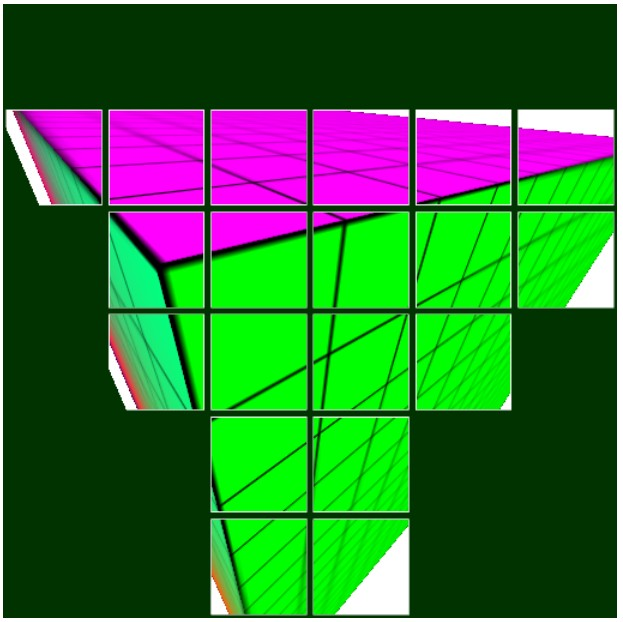
\includegraphics[width=.3\linewidth]{splat1.jpg}
  }
  \subfigure[$P_c M_c = P_s M_s$]{
    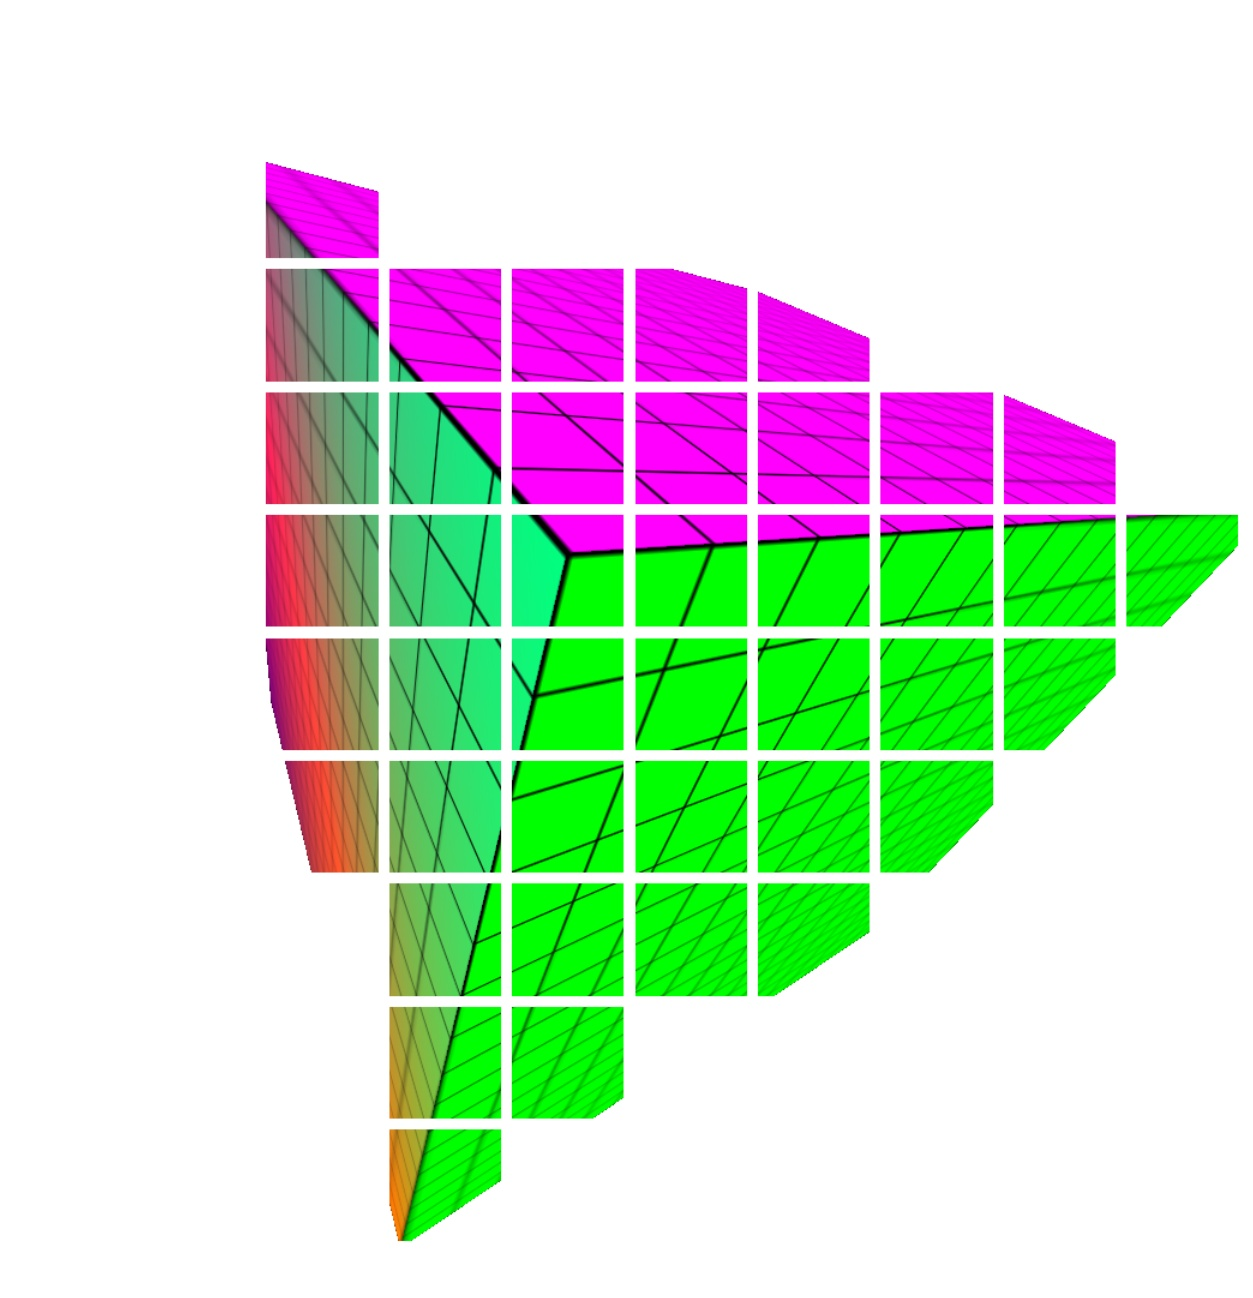
\includegraphics[width=.3\linewidth]{splat2.jpg}
  }
  \subfigure[$P_c M_c \neq P_s M_s$]{
    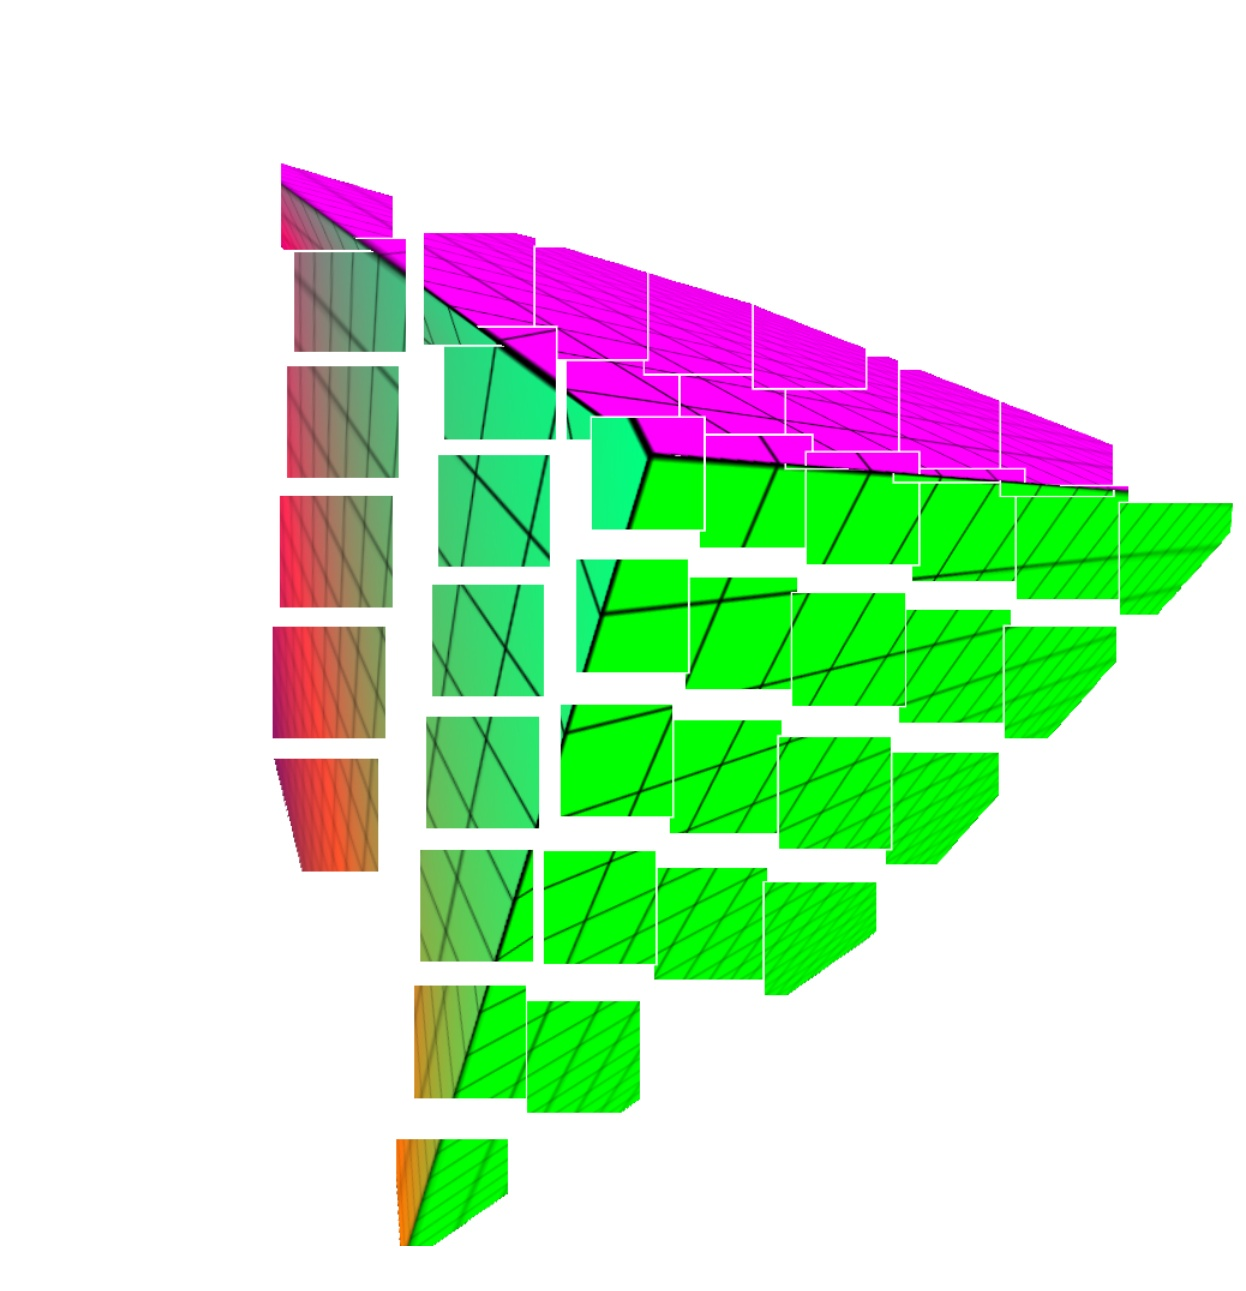
\includegraphics[width=.3\linewidth]{splat3.jpg}
  }
  \caption{\label{fig:LargeSplatsOnCorners}
           Splats for which depths are sampled on a planar region look nice on
  this region, but possibly contorted elsewhere. Notice the corner and edges
  here, where we have chosen parameters to display this effect.}
\end{figure}

When the geometry is not planar, $T$ produces the wrong result for parts of a
splat.  Two ways to remedy this could be to choose either more and smaller
splats, or introduce more complex texture transformations. Note that using a
more sophisticated texture coordinate transform may amount to performing the
same work as for more and simpler transforms. The latter may be regarded as
exactly a better ``global'' texture transform implementation.


%-------------------------------------------------------------------------
\subsubsection{Other splat considerations}
\label{sec:proxyModelReplacement}

\textbf{Splat sizing} 
Each splat should be rendered into a number of client pixels according to the
new splats' 3D position. To achieve this, we use the vectors $\sv_{\Delta x}$
and $\sv_{\Delta y}$ from the previous section, and in addition, we scale the
splats up a bit so that they overlap. Hence, we can render rectangular
window-aligned splats with less risk of getting uncovered areas when
interactively rotating and scaling the model on the client. In most cases this
removes the problem visualized in Figure~\ref{fig:LargeSplatsOnCorners}.

\textbf{Splat depth fragments}
For larger splats it makes sense to also compute and use depth fragments on the
client. The ``intra-splat'' depth values can easily be fetched from the depth
image, just as the texture is looked up for color. Not all clients support this
WebGL extension.

\textbf{Splat set replacement algorithms}
We mainly concern ourselves with proxy models defined as sets of splats, and it
makes sense to keep a set of such models on the client, then we may combine them
to cover larger ranges of client-side transformations. One can imagine a plethora of
{\em splat set replacement algorithms}, we have tested three approaches that all
retain a constant number of proxy models. The first is to replace the
one with a viewing direction differing the most from the newly received
model. The second simply replaces the oldest one in store. The third replaces a
proxy model $k$ if the replacement results in the following objective function
being reduced,
\begin{equation}
  \text{coverage} =
  \sum_{i=1}^n
    \sum_{j\neq i}^n 
      ( \angle(\textbf{camdir}_i, \textbf{camdir}_j )^2,
  \label{eq:coverage}
\end{equation}
where $n$ is the number of proxy models available, $\textbf{camdir}$ is the
direction in which the camera was looking when a particular model was generated,
and the model to be replaced is the one that minimizes~(\ref{eq:coverage}) after
replacement.


%-------------------------------------------------------------------------
\subsection{Auto-tuning}
\label{sec:autoTuning}

It is important that the process of generating and sending proxy model data from
the server itself does not slow down transmission.  There are mainly three
sources of delay for server-rendered images to the client; high latency, low
bandwidth, and slow server-rendering.  In the first case, it seems prudent to
have a good proxy model on the client, which can be used for longer time and for
a wider range of client-side transformations.  In the two other cases, it is
important for the proxy model generation/transmission to be cheap/fast, both in order
to get the proxy model to the client and keep from delaying the server-image
more than necessary. These demands are not always compatible.

We have adopted an adaptive specification of proxy model data from the server
involving a more light-weight image (lossy JPG-compression with adaptive quality
control) while interaction is ongoing.  Also, reduced resolution of the depth
buffer sent from the server is used. Another possibility is to let the client
dynamically set the number of splats, number of proxy models, etc.


%-------------------------------------------------------------------------
\section{Results and discussion}

We have tested the algorithms discussed in the ZZZZ (name withheld for the
double-blind review process) framework, which is a programming framework for
setting up and managing client/server based interactive visualization
applications, see~\cite{tinia}. As client we use Google Chrome, code is written
in standard Javascript/WebGL.  The implementation in ZZZZ is invisible to the
application, so all existing ZZZZ-applications will have the feature
available. The algorithm is minimally intrusive in that only the depth buffer
will have to be added to the rendering output of the application. We have tested
several smaller test cases, but also on a larger oil reservoir viewer,
YYYY~\cite{cloudviz}.

YYYY utilizes several GLSL shaders to render reservoir cells, boundaries,
tubular wells etc., and visualizes a 3D model that is not trivial to reduce in
complexity. It is typically also very large, so rendering it on a thin client is
prohibitive. With the automatic proxy model, we obtain interactive frame rates
with limited connection from a lightweight client. For a comparison of a
server-rendered image and a client-rendered proxy model that is slightly rotated
on the client, see again Figure~\ref{fig:FRView}. In
Figure~\ref{fig:FRView}~(a), the full server-rendered image is shown, and in~(b)
and~(c), a slightly (about 10 degrees) rotated proxy model is rendered on the
client. In~(b), parameters are chosen for best possible results, while in~(c),
we want to highlight effects, so it uses a small number of non-overlapping large
splats. One can easily spot areas not well covered, and areas where the texture
coordinate transform $T$ does not produce optimal results.



%-------------------------------------------------------------------------
\section{Conclusion and future work}

The most attractive feature of the method described is the automated generation
of the proxy model. Problems with compression and simplification of existing
geometries is bypassed altogether. The automatic proxy model implementation is
invisible to the application. There are several directions in which we would
like to follow up and improve this concept, a couple of these are,
\begin{itemize}

\item \textbf{Proxy model replacement algorithms} Obtaining good results with a minimal set of
proxy models.

\item \textbf{Depth compression} We would like to ivestigate other approaches
than just truncation, see \eg,~\cite{DBLP:journals/tvcg/Lindstrom14}.

\item \textbf{Deferred shading} With a normal map more advanced
shading could be done on the client. Such a map could also be constructed from
the depth map.

\end{itemize}


%-------------------------------------------------------------------------

%\bibliographystyle{eg-alpha}
\bibliographystyle{eg-alpha-doi}

\bibliography{egbibsample}

%-------------------------------------------------------------------------

\end{document}
